% !TEX root = main.tex

\chapter{Overview}
\label{ch:overview}
\noindent


\begin{figure}[h]
  \centerline{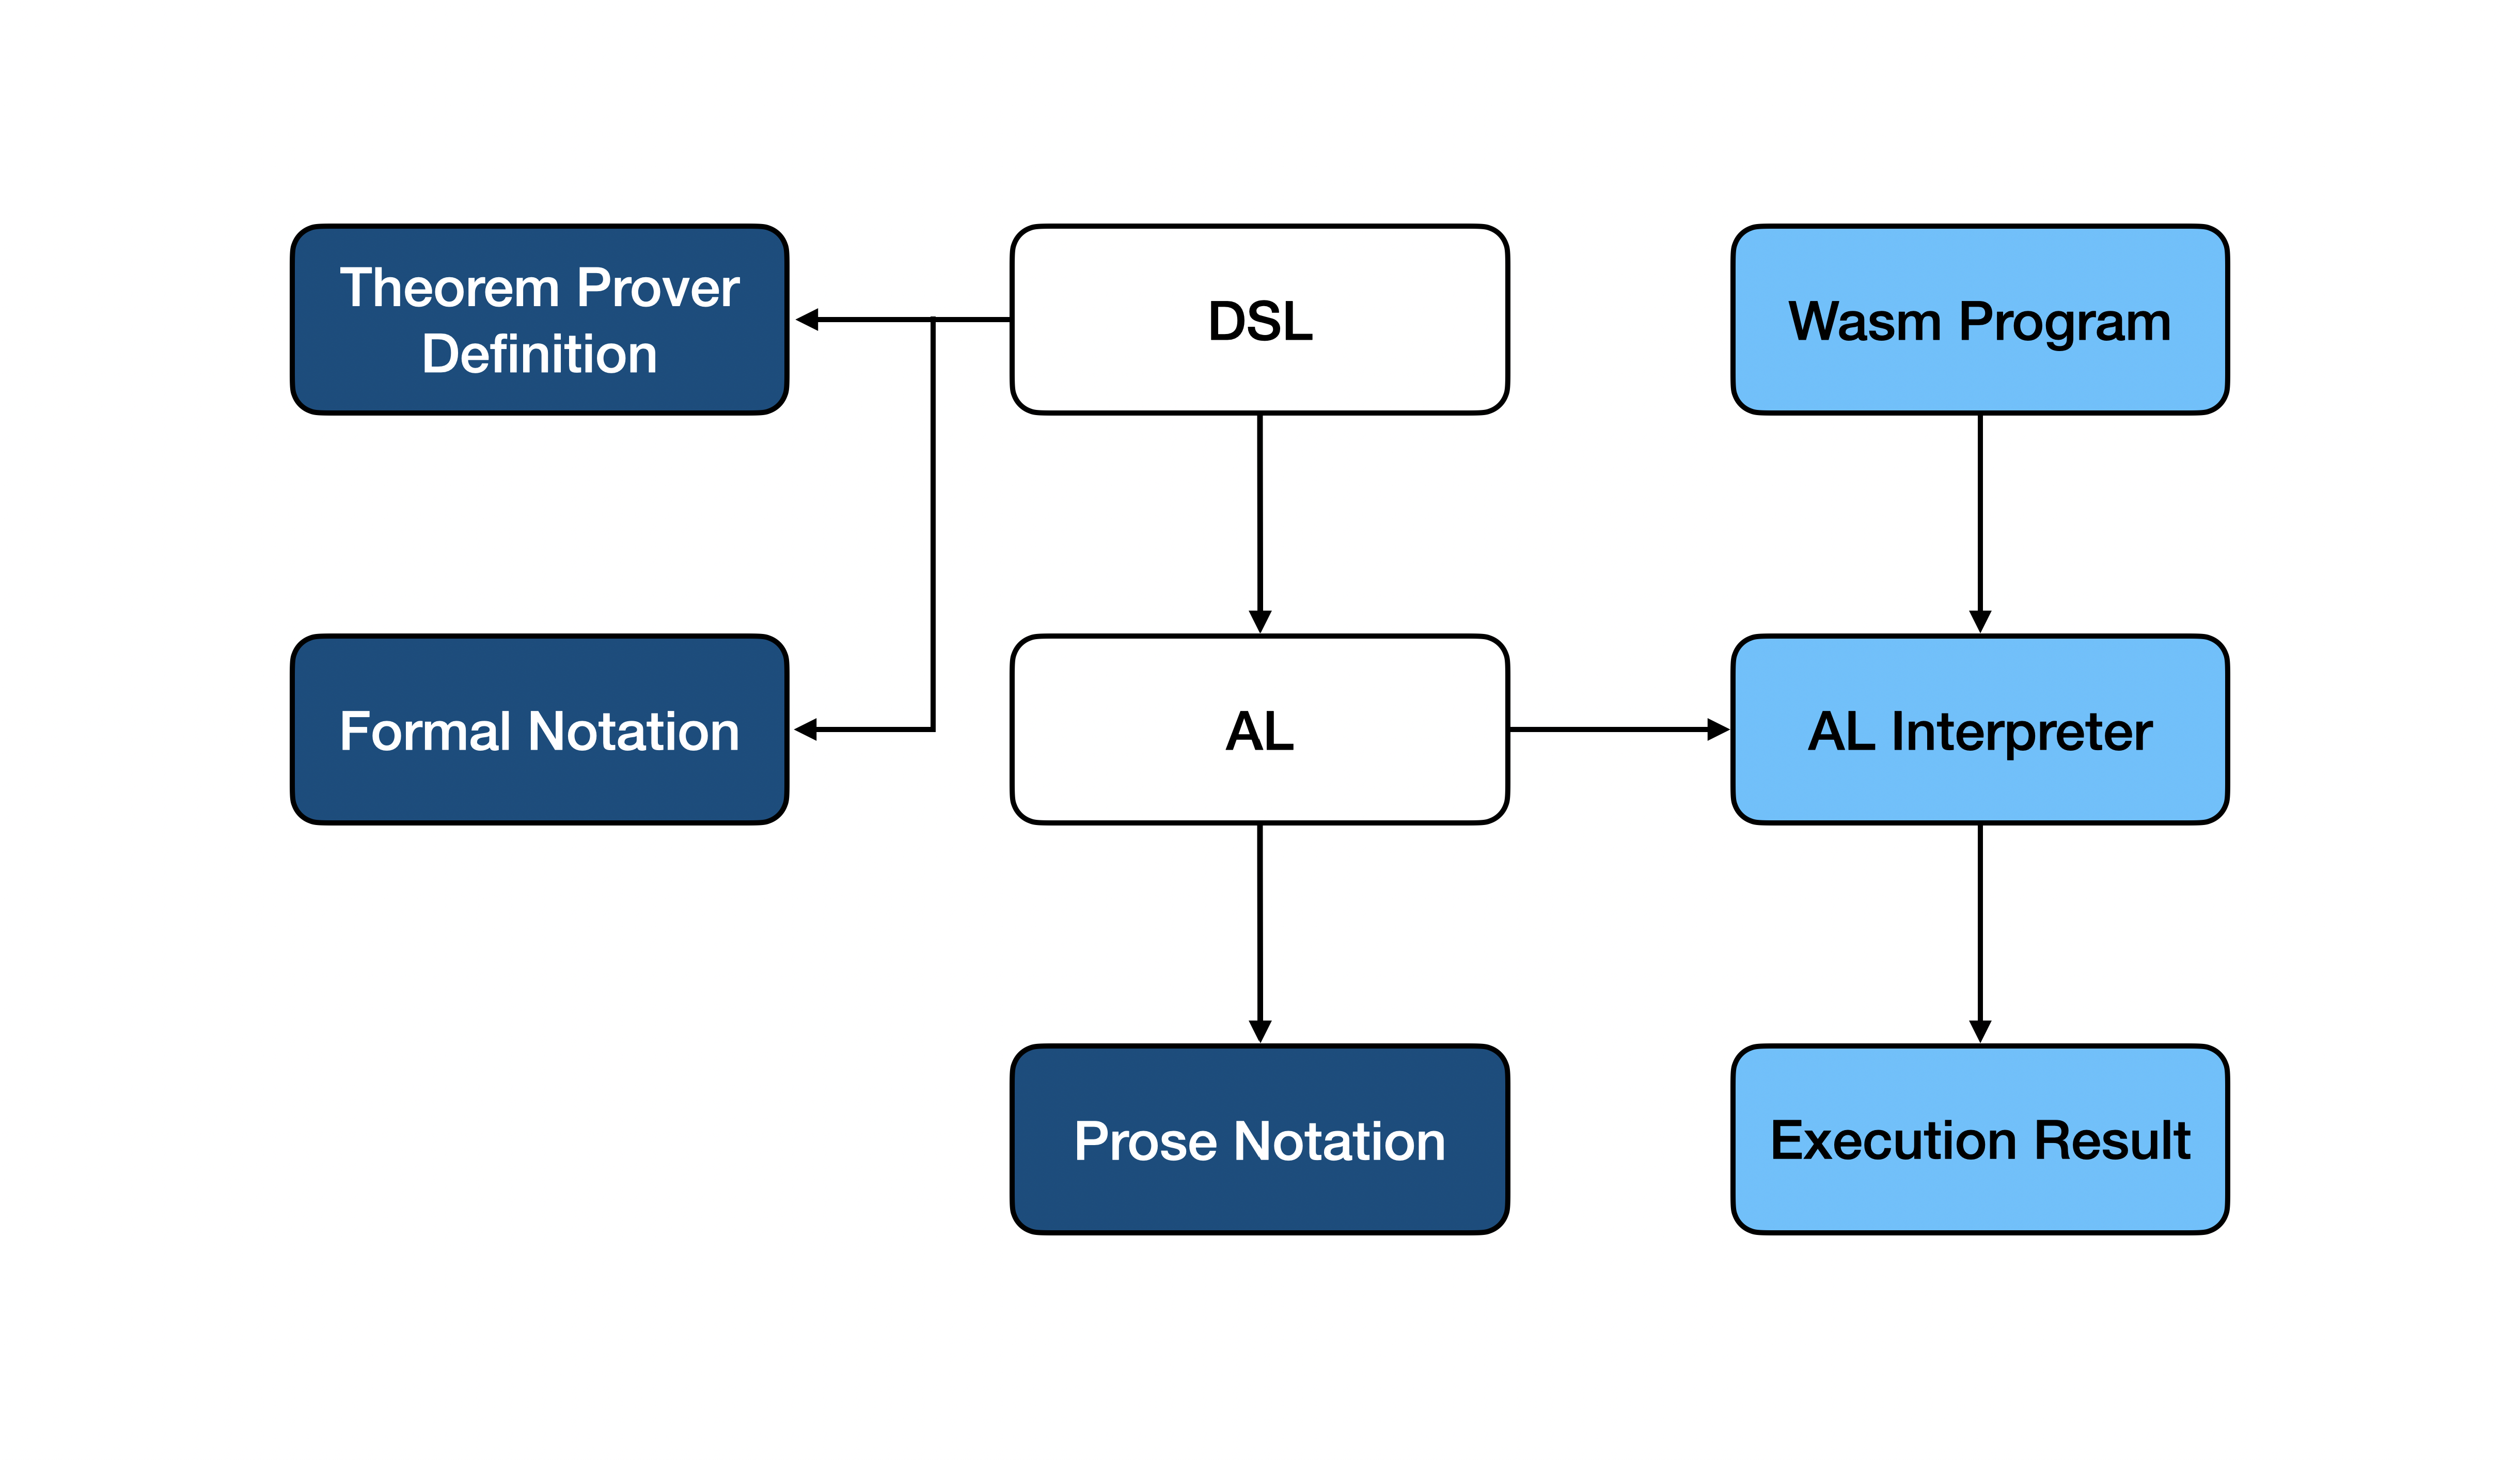
\includegraphics[width=15cm]{fig/overview}}
  \caption[An overview of the SpecTec architecture]
    {An overview of the SpecTec architecture}
    \label{fig:overview}
\end{figure}

% Overview explanation
In this chapter, we explain an overall approach to generate multiple artifacts
from the specification and check correctness of the specification.
\cref{fig:overview} illustrates the overview of our approach.
SpecTec provides a domain specific language (DSL) for the specification.
It is designed to be similar to the formal notation when describing the
semantics with compact and user-friendly notation.
It is type checked to prevent meta-level errors such as notation misuses and
dimension mismatches.
The code below is the specification for \texttt{testop} instruction written in
the DSL.
\begin{lstlisting}[escapechar=\%]
  rule Step_pure/testop:
  (CONST nt c_1) (TESTOP nt testop)  %$\codetilde$%>  (CONST I32 c)
  -- if c = %$\codedollar$%testop_(nt, testop, c_1)
\end{lstlisting}
